\chapter{Likelihood} 

This chapter contains notes on how likelihoods are calculated in Phycas. All of this discussion concerns the C++ code, not the Python code, which simply wraps the C++ functions. This documentation does not get into the real nitty-gritty, but instead is designed as an overview; if you want to know the details see the bodies of the functions referenced.

%%%%%%%%%%%%%%%%%%%%%%%%%%%%%%%%%%%%%%%%%%%%%%%%%%%%%%%%%%%%%%
%%%%%%%%%%%%%%%%%%%%%%%%%%%%%%%%%%%%%%%%%%%%%%%%%%%%%%%%%%%%%%
\section{Definitions of terms and acronyms}
%%%%%%%%%%%%%%%%%%%%%%%%%%%%%%%%%%%%%%%%%%%%%%%%%%%%%%%%%%%%%%
%%%%%%%%%%%%%%%%%%%%%%%%%%%%%%%%%%%%%%%%%%%%%%%%%%%%%%%%%%%%%%
\begin{description}
\item[CLA] Conditional Likelihood Array. This is a vector containing the likelihood of a subtree at a particular site and given a particular state and rate (if using a rate heterogeneity mixture model). Each edge in the tree has potentially two CLAs, one pointing in each direction. The CLAs are stored in a pool and reused to avoid excessive construction/destruction costs.
\item[invalidate] A node is said to be invalidated when the CLAs for its edge are stored in the pool. This means that the next time the likelihood needs to be calculated, the CLAs will need to be recalculated for this node. Invalidation occurs when a parameter that affects all CLAs is changed, or if the edge length for a node changes. 
\item[subroot] This is the node just above the node at which the tree is rooted. (Perhaps epiroot would be a better term for this.) The subroot node has just one parent (the root node) and thus the root node just has one child (the subroot node).
\end{description}

%%%%%%%%%%%%%%%%%%%%%%%%%%%%%%%%%%%%%%%%%%%%%%%%%%%%%%%%%%%%%%
%%%%%%%%%%%%%%%%%%%%%%%%%%%%%%%%%%%%%%%%%%%%%%%%%%%%%%%%%%%%%%
\section{Data structures used in calculating likelihoods}
%%%%%%%%%%%%%%%%%%%%%%%%%%%%%%%%%%%%%%%%%%%%%%%%%%%%%%%%%%%%%%
%%%%%%%%%%%%%%%%%%%%%%%%%%%%%%%%%%%%%%%%%%%%%%%%%%%%%%%%%%%%%%

\subsection{Conditional likelihood arrays (CLAs)}

Here is the layout of a conditional likelihood array. In this case, the data is partitioned into two subsets, the first with 10 DNA characters (and a model that specifies 3 rate categories) and the second comprises 3 2-state morphological characters (no rate heterogeneity).

THE LAYOUT BELOW IS INCORRECT - PATTERNS ARE NESTED WITHIN RATES!

\resizebox{5.5in}{!} {
\begin{tabular}{|c|c|c|c|c|c|c|c|c|c|c|c|c|c|c|c|c|c|c|c|c|c|c|c|c|c|c|c|c} \hline
\multicolumn{12}{|c|}{Pattern 1} & \multicolumn{12}{c|}{Pattern 2} & \multicolumn{5}{c}{} \\ \hline
\multicolumn{4}{|c|}{Rate 1} & \multicolumn{4}{c|}{Rate 2} &\multicolumn{4}{c|}{Rate 3} &
\multicolumn{4}{c|}{Rate 1} &\multicolumn{4}{c|}{Rate 2} &\multicolumn{4}{c|}{Rate 3} &\multicolumn{4}{c|}{Rate 1} & \\ \hline
A & C & G & T & A & C & G & T & A & C & G & T & A & C & G & T & A & C & G & T & A & C & G & T & A & C & G & T & A \\ \hline
\multicolumn{4}{c}{} & \multicolumn{1}{c}{$\uparrow$} &   \multicolumn{24}{c}{} 
\end{tabular}
}
$\cdots$

$\cdots$
\resizebox{3.5in}{!} {
\begin{tabular}{|c|c|c|c|c|c|c|c|c|c|c|c|c|c|c|c|c|c|} \hline
\multicolumn{12}{|c|}{Pattern 10} & \multicolumn{2}{|c|}{11} & \multicolumn{2}{|c|}{12} & \multicolumn{2}{|c|}{13} \\ \hline
\multicolumn{4}{|c|}{Rate 1} & \multicolumn{4}{c|}{Rate 2} & \multicolumn{4}{c|}{Rate 3} & \multicolumn{2}{c|}{} & \multicolumn{2}{c|}{} & \multicolumn{2}{c|}{} \\ \hline
A & C & G & T & A & C & G & T & A & C & G & T & 0 & 1 & 0 & 1 & 0 & 1 \\ \hline
\end{tabular}
}

Note that a single conditional likelihood array spans all partition subsets. It is therefore not possible to determine the length of the CLA by multiplying $(\mbox{no. patterns})\times(\mbox{no. rates})\times(\mbox{no. states})$ because (no. rates) and (no. states) can differ between partition subsets.

The element indicated by the arrow represents the probability of data pattern 1 ``above'' this node given that the relative rate was 2 and this node had state A. ``Above'' is in quotes because it is possible that the likelihood root is a descendant of the focal node, in which case the subtree involved may be pointing down rather than up. Note that nothing special need be done to accommodate partitioning; different models are being used here to compute the conditional likelihood for pattern 10 vs. pattern 11, for example.

The CLAs are managed by the ConditionalLikelihood class. The InternalData and TipData classes each have a data member {\tt cla\_pool} that stores a stack of ConditionalLikelihood objects. Each InternalData object also has four ConditionalLikelihood shared pointers: {\tt parWorkingCLA} and {\tt parCachedCLA} store CLAs that are valid for subtrees rooted at the parent node, while {\tt childWorkingCLA} and {\tt childCachedCLA} store CLAs that are valid for subtrees rooted at the node that owns them. The ``cached'' versions allow temporary storage for use during Metropolis-Hastings proposals; if a proposed move is rejected, the cached versions are swapped back in rather than being recalculated. TipData objects have only the {\tt parWorkingCLA} and {\tt parCachedCLA} data members.

\subsection{Transition matrix arrays}

The InternalData and TipData classes have a data member {\tt pMatrices} that is a ScopedThreeDMatrix. The first dimension ranges over representative relative rates, so {\tt pMatrices[r]} provides a 2-dimensional transition probability matrix for the rate category {\tt r}. Here is how {\tt pMatrices} is laid out in the ScopedThreeDMatrix object pointed to by an InternalData object's {\tt pMatrices} data member:

\resizebox{5.5in}{!} {
\begin{tabular}{cccccccccccccccc}
      &    & \multicolumn{4}{c}{to state} & & \multicolumn{4}{c}{to state} & & \multicolumn{4}{c}{to state}	\\
      &    & A  & C  & G  &  T & & A  & C  & G  &  T & & A  & C  & G  &  T \\  \cline{3-6} \cline{8-11} \cline{13-16}
      &  A & \multicolumn{1}{|c}{0} & 1  & 2  &  \multicolumn{1}{c|}{3} & & \multicolumn{1}{|c}{16} & 17 & 18 & \multicolumn{1}{c|}{19} & & \multicolumn{1}{|c}{32} & 33 & 34 & \multicolumn{1}{c|}{35} \\
from  &  C & \multicolumn{1}{|c}{4} & 5  & 6  &  \multicolumn{1}{c|}{7} & & \multicolumn{1}{|c}{20} & 21 & 22 & \multicolumn{1}{c|}{23} & & \multicolumn{1}{|c}{36} & 37 & 38 & \multicolumn{1}{c|}{39} \\
state &  G & \multicolumn{1}{|c}{8} & 9  & 10 &  \multicolumn{1}{c|}{11} & & \multicolumn{1}{|c}{24} & 25 & 26 & \multicolumn{1}{c|}{27} & & \multicolumn{1}{|c}{40} & 41 & 42 & \multicolumn{1}{c|}{43} \\
      &  T & \multicolumn{1}{|c}{12} & 13 & 14 & \multicolumn{1}{c|}{15} & & \multicolumn{1}{|c}{28} & 29 & 30 & \multicolumn{1}{c|}{31} & & \multicolumn{1}{|c}{44} & 45 & 46 & \multicolumn{1}{c|}{47} \\ \cline{3-6} \cline{8-11} \cline{13-16}
      &    & \multicolumn{4}{c}{rate 1} & & \multicolumn{4}{c}{rate 2} & & \multicolumn{4}{c}{rate 3}	\\
\end{tabular}
}

The number in each cell shows the position in memory: all elements in a ScopedThreeDMatrix are laid out in contiguous memory for reasons of cache efficiency. The transition probability matrices in TipData structures are different because they are transposed (rows are the ``to'' states, columns are the ``from'' states, and are augmented with extra rows to deal with ambiguities.

%|				|--------------- from state -------------|
%|					0		   1		  2			 3
%|					A		   C		  G			 T
%|	t  0   A	 0.90638	0.03121	   0.03121	  0.03121
%|	o  1   C	 0.03121	0.90638	   0.03121	  0.03121
%|	   2   G	 0.03121	0.03121	   0.90638	  0.03121
%|	s  3   T	 0.03121	0.03121	   0.03121	  0.90638
%|	t  4   N	 1.00000	1.00000	   1.00000	  1.00000 \
%|	a  5 {GT}	 0.06241	0.06241	   0.93759	  0.93759  | These rows not present if prepareForSimulation function
%|	t  6 {ACT}	 0.96879	0.96879	   0.09362	  0.96879  | was used to create the TipData structures
%|	e  7 {AG}	 0.93757	0.06241	   0.93759	  0.06241 /


%%%%%%%%%%%%%%%%%%%%%%%%%%%%%%%%%%%%%%%%%%%%%%%%%%%%%%%%%%%%%%
%%%%%%%%%%%%%%%%%%%%%%%%%%%%%%%%%%%%%%%%%%%%%%%%%%%%%%%%%%%%%%
\section{Functions for computing likelihoods}
%%%%%%%%%%%%%%%%%%%%%%%%%%%%%%%%%%%%%%%%%%%%%%%%%%%%%%%%%%%%%%
%%%%%%%%%%%%%%%%%%%%%%%%%%%%%%%%%%%%%%%%%%%%%%%%%%%%%%%%%%%%%%

\subsection{TreeLikelihood::calcLnL}
This function is the one to call to get a likelihood calculated. It takes a shared pointer to a Tree and returns a double (the log-likelihood). It first determines which node should serve as the root of the likelihood calculation (and this need not be, and usually isn't, the root of the tree). If the data member {\tt likelihood\_root} is NULL, the entire tree is invalidated (all CLAs are stored) and the likelihood root is set to the subroot node. If the data member {\tt likelihood\_root} points to a node, that node will be used as the root of the likelihood calculation. This function then calls either calcUnimapLnL or calcLnLFromNode (depending on the state of {\tt using\_unimap}) to do the work.

%
% Figure "edgeiterator"
%
\begin{figure}[t]
\begin{center}
\hfil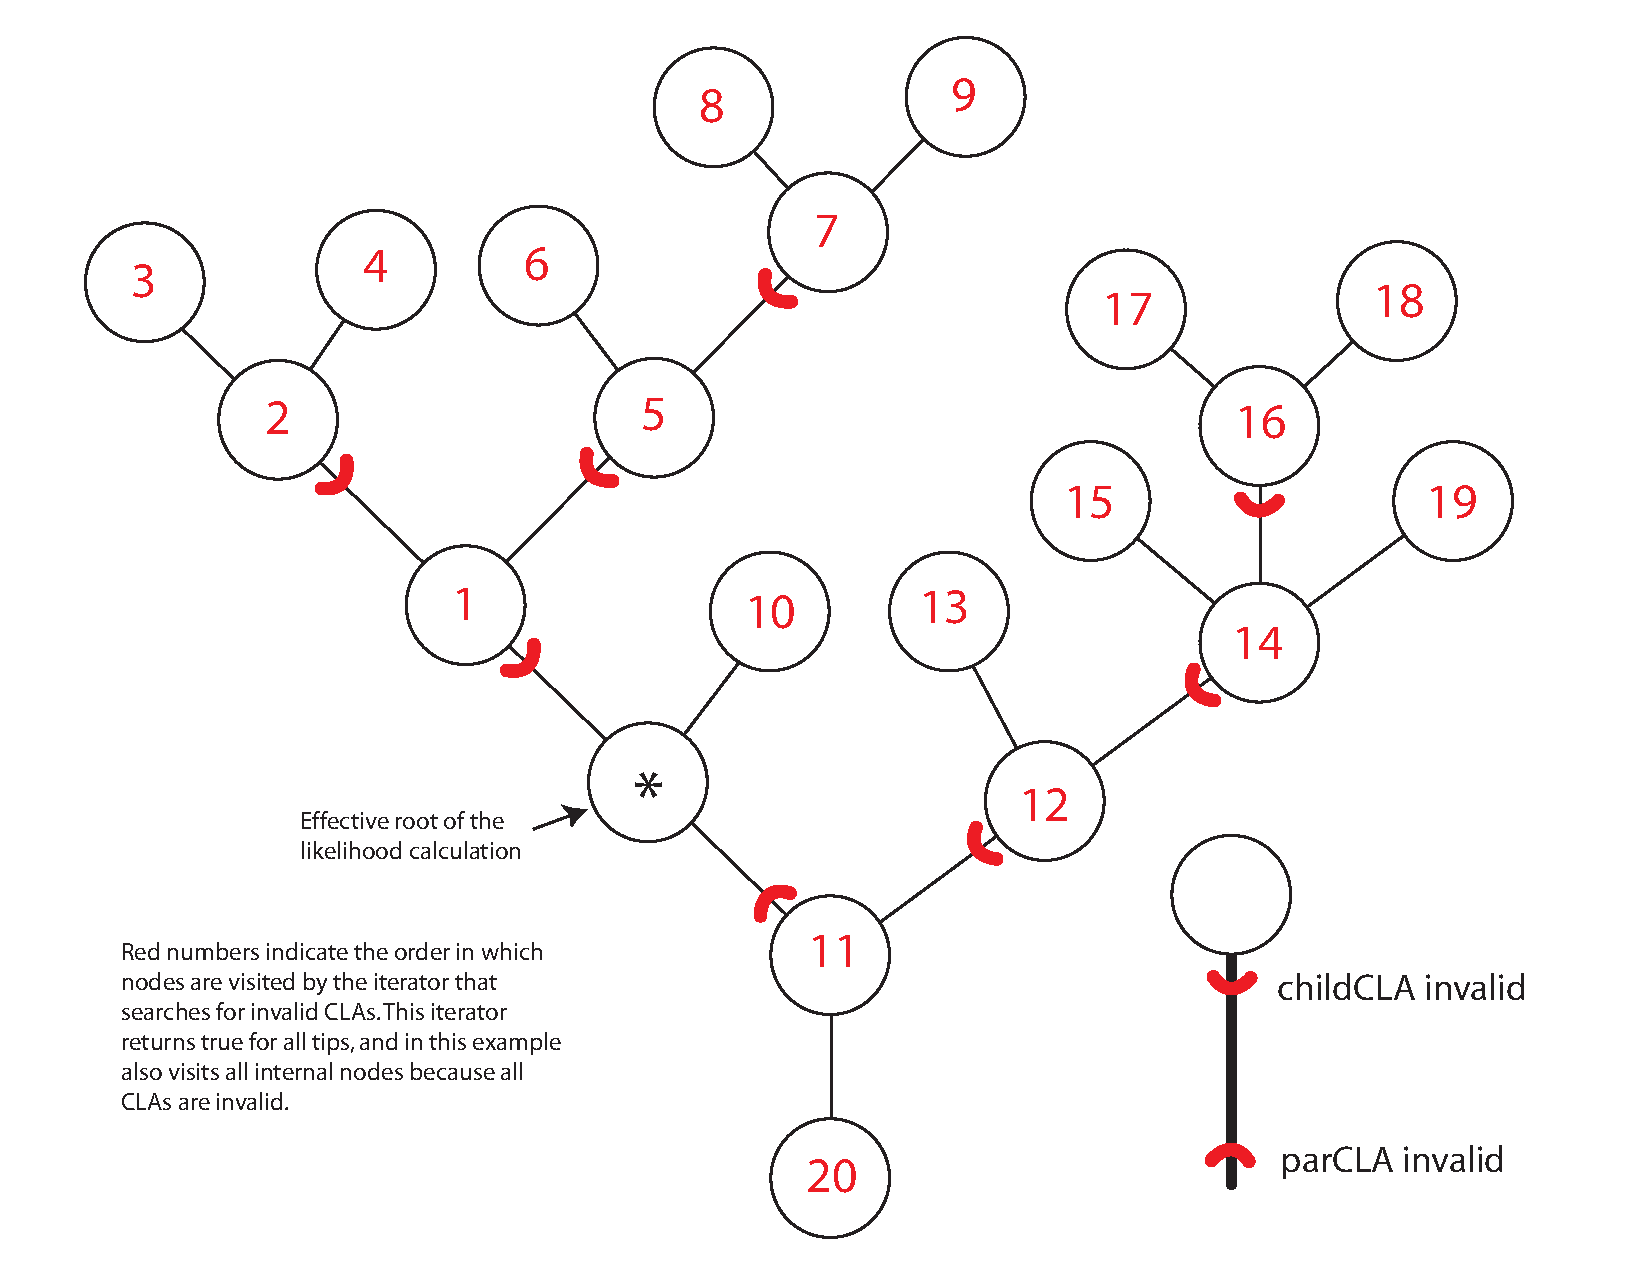
\includegraphics[scale=0.6]{ConditionalLikelihoodArrays/EffectiveRoot.pdf}\hfil
\caption{Order in which nodes are visited by the effective\_postorder\_edge\_iterator in the process of building a stack of nodes for which the TreeLikelihood::refreshCLA function is called.}
\label{edgeiterator}
\end{center}
\end{figure}

\subsection{TreeLikelihood::calcLnLFromNode}
If {\tt no\_data} is true, returns 0.0; otherwise, calls refreshCLA to update the CLAs that are invalid and then returns the value returned by the harvestLnL function. The effective\_postorder\_edge\_iterator is used to iterate through nodes for which refreshCLA needs to be called. This iterator first visits nodes in a centrifugal fashion away from the focal node, building a stack of nodes that need to have their CLAs recalculated. See Figure~\ref{edgeiterator} for an illustration of this process showing the order in which nodes are visited by the iterator in this first sweep to build the stack. Then, it pops nodes off this stack and hands them to the refreshCLA function. So CLAs are recalculated in a centripetal order (this would be equivalent to a postorder traversal if the likelihood root were equal to the actual root of the tree).

\subsection{TreeLikelihood::refreshCLA}
This function takes a reference to a focal node and a pointer to a node to avoid. It recalculates the CLA for the focal node in a direction away from the avoid node. The CLA is computed based on two nodes adjacent to the focal node, called firstNeighbor and secondNeighbor. If the path from the focal node to the likelihood root would go through the focal node's parent, then firstNeighbor is the leftmost child of the focal node and secondNeighbor is its right sibling, otherwise firstNeighbor is the parent of the focal node and secondNeighbor is the leftmost child that is not the avoid node. The necessary transition probability matrices are computed using one of two functions: calcPMat is used for internal nodes and calcPMatTranspose is used for tips. One of three functions (calcCLANoTips, calcCLAOneTip, calcCLATwoTips) is then called depending on the status of firstNeighbor and secondNeighbor. If secondNeighbor has siblings that are not equal to the avoided node, then the focal node represents a polytomy and either conditionOnAdditionalTip or conditionOnAdditionalInternal must be called for each extra sibling. Figure~\ref{edgeiterator} illustrates the CLAs that would be recomputed by this function in an example tree where the likelihood root is not equal to the actual root and no CLAs are currently valid.

\subsection{TreeLikelihood::calcPMat}

This function defers everything to calcPMatCommon.
\partition{First argument is now the subset index.}

\subsection{TreeLikelihood::calcPMatCommon}

Creates a vector of scaled edge lengths, each element of which is the edge length multiplied by a relative rate mean. It then passes a pointer to the beginning of this vector to the model's calcPMatrices function to do the work.
\partition{First argument is now the subset index.}

\subsection{TreeLikelihood::calcPMatTranspose}
\partition{First argument is now the subset index.}

\subsection{TreeLikelihood::calcCLAOneTip}

\subsection{TreeLikelihood::calcCLATwoTips}

\subsection{TreeLikelihood::conditionOnAdditionalTip}

\subsection{TreeLikelihood::conditionOnAdditionalInternal}

\subsection{TreeLikelihood::harvestLnL}

By the time harvestLnL is called, all CLAs are up-to-date. Normally, the sole argument is an EdgeEndpoints object in which the focal node is specified to be the likelihood root and the focal neighbor is NULL. In this case, the focal neighbor is set to be the parent of the focal node. The refreshCLA function is then called to refresh the childCLA of the focal node (i.e. its parent is specified as the avoid node). A new ConstEdgeEndpoints object is created and passed to harvestLnLFromValidEdge for processing.

\subsection{TreeLikelihood::harvestLnLFromValidEdge}

This function computes the log-likelihood (and site likelihoods if {\tt store\_site\_likes} is true) over all patterns. It is assumed that the focal node is an internal node. If the focal neighbor is a tip node, then the overall likelihood for pattern $k$ is
\begin{eqnarray*}
L_k & = & \sum_r \sum_{s_f} \pi_{s_f} P(s_f|s_n,r) L(f|s_f,r),
\end{eqnarray*}
where $L(f|s_f,r)$ is the likelihood conditional on state $s_f$ at the focal node for rate $r$, $\pi_{s_f}$ is the relative frequency of state $s_f$, and $P_{s_n|s_f,r}$ is the transition probability of ending in state $s_n$ given starting state $s_f$ for rate $r$. Note that Phycas uses the transition matrix backwards here ($P_{s_f|s_n,r}$ instead of $P_{s_n|s_f,r}$), which is ok as long as the model is time-reversible (and it must be time-reversible if the focal neighbor is a tip).

If the focal neighbor is an internal node, then the overall likelihood for pattern $k$ is instead
\begin{eqnarray*}
L_k & = & \sum_r \sum_{s_f} L(f|s_f,r) \left\{ \sum_{s_n} \pi_{s_f} P(s_n|s_f,r) L(n|s_n,r) \right\},
\end{eqnarray*}
where $L(f|s_f,r)$ is the likelihood conditional on state $s_f$ at the focal node for rate $r$, $L(n|s_n,r)$ is the likelihood conditional on state $s_n$ at the focal {\em neighbor} node for rate $r$, $\pi_{s_f}$ is the relative frequency of state $s_f$, and $P_{s_n|s_f,r}$ is the transition probability of ending in state $s_n$ given starting state $s_f$ for rate $r$. The quantity $\pi_{s_f} P(s_n|s_f,r)$ is precalculated and stored in {\tt piP[r][s\_f][s\_n]}, where {\tt piP} is a 3-dimensional temporary matrix. This is done to avoid recalculating the product of state frequency and transition probability for each pattern. This also explains why the $\pi_{s_f}$ is inside the $s_n$ loop.

For pinvar models, there is additional code to compute the likelihood of a pattern given that it is invariable. This work is only done if the pattern is potentially constant. There is also code for computing the correction for underflow. Finally, to obtain the site log-likelihood, the log-likelihood for each pattern is multiplied by the count for that pattern.


